\documentclass[a4paper,11pt]{article}

	%% From https://github.com/aytchell/latex-listings-protobuf/tree/09c39676e6afb2af8c7d21ed21a516359c52e27c/

\usepackage{xcolor}
\usepackage{xcolor-solarized}
\usepackage{textcomp}

\newcommand{\SetProtoColorsSolarized}{
  % Colors taken from the 'solarized' color scheme of Ethan Schoonover
  % (with light background)
  % http://ethanschoonover.com/solarized
  \colorlet{proto_basic}{solarized-base00}
  \colorlet{proto_keyword}{solarized-cyan}
  \colorlet{proto_type}{solarized-cyan}
  \colorlet{proto_options}{solarized-cyan}
  \colorlet{proto_comment}{solarized-base1}
  \colorlet{proto_string}{solarized-blue}
  \colorlet{proto_number}{solarized-violet}
  \colorlet{proto_ident}{solarized-base00}
  \colorlet{proto_digits}{solarized-violet}
  \colorlet{proto_background}{solarized-base3}
}

\newcommand{\SetProtoColorsBlueish}{
  % Colors inspired by the NASM style of Robin Eklind
  % https://github.com/mewspring/latex
  \definecolor{proto_basic}{RGB}{0,0,0}             % black
  \definecolor{proto_keyword}{RGB}{0,0,0}         % black
  \definecolor{proto_ident}{RGB}{128,0,0}            % dark red
  \definecolor{proto_options}{RGB}{128,0,128}       % purple
  \definecolor{proto_comment}{RGB}{0,128,0}         % dark green
  \definecolor{proto_string}{RGB}{255,0,0}          % red
  \definecolor{proto_number}{RGB}{108,113,196}      % violet
  \definecolor{proto_type}{RGB}{0,0,255}             % blue
  \definecolor{proto_digits}{RGB}{0,0,128}          % dark blue
  \definecolor{proto_background}{RGB}{255,255,255}  % white
}

\newcommand{\SetProtoColorsTomorrow}{
  % Colors taken from the 'Tomorrow' color scheme of Chris Kempson
  % https://github.com/chriskempson/tomorrow-theme/blob/master/vim/colors/Tomorrow.vim
  \definecolor{proto_basic}{RGB}{77, 77, 76}          % dark grey
  %\definecolor{proto_keyword}{RGB}{245, 135, 31}      % orange
  \definecolor{proto_keyword}{RGB}{66, 113, 174}      % orange
  %\definecolor{proto_type}{RGB}{66, 113, 174}         % purple
  \definecolor{proto_type}{RGB}{200, 40, 41}         % red
  \definecolor{proto_options}{RGB}{137, 89, 168}
  %\definecolor{proto_comment}{RGB}{142, 144, 140}     % gray
  \definecolor{proto_comment}{RGB}{0,0,0}             % black
  \definecolor{proto_string}{RGB}{113, 140, 0}        % green
  \definecolor{proto_number}{RGB}{137, 89, 168}
  %\definecolor{proto_ident}{RGB}{200, 40, 41}         % red
  \definecolor{proto_ident}{RGB}{0,128,0}           % dark green
  \definecolor{proto_digits}{RGB}{245, 135, 31}       % orange
  \definecolor{proto_background}{RGB}{255, 255, 255}  % white
}

%\SetProtoColorsSolarized{}
\SetProtoColorsTomorrow{}
%\SetProtoColorsBlueish{}

\lstdefinestyle{protobuf}{
  frame=lines,
  %xleftmargin=\parindent,
  belowcaptionskip=1\baselineskip,
  backgroundcolor=\color{proto_background},
  basicstyle=\color{proto_basic}\footnotesize\ttfamily,
	keywordstyle=[1]\color{proto_keyword},
	keywordstyle=[2]\color{proto_type},
	keywordstyle=[3]\color{proto_options},
	commentstyle=\color{proto_comment},
	stringstyle=\color{proto_string},
  numberstyle=\color{proto_ident}\tiny,
  identifierstyle=\color{proto_ident}\bfseries,
	numbers=none, %left,
	numbersep=5pt,
	breaklines=false,
	showstringspaces=false,
	tabsize=2,
	prebreak=\raisebox{0ex}[0ex][0ex]{\ensuremath{\hookleftarrow}},
	upquote=true,
}

	
        \usepackage[notes=true]{lib/dtrt}
	\usepackage{algorithm}
	\usepackage{algpseudocode}
	\usepackage{amsmath}
	\usepackage{xcolor}
	\usepackage{graphicx}
	\usepackage{todonotes}
	\usepackage{listings}
	\usepackage{pxfonts}
	\usepackage[margin=1in]{geometry}

	\usepackage{lib/lang}  % include language definition for protobuf
	\usepackage{lib/style} % include custom style for proto declarations.	
	
	%\usepackage{sagetex}

	% Auuthor notes (using dtrt's macros). Switch the dtrt package flag to notes=false to hide.
	\definecolor{darkgreen}{rgb}{0,0.6,0}
	\newcommand{\dnote}[1]{\dtcolornote[Daniel]{red}{#1}}
	\newcommand{\anote}[1]{\dtcolornote[Aurell]{blue}{#1}}
	\newcommand{\enote}[1]{\dtcolornote[Eran]{darkgreen}{#1}}

	\newcommand\dtodo[1]{\todo[color=red!20]{#1}}
	\newcommand\atodo[1]{\todo[color=green!20]{#1}}
	\newcommand\etodo[1]{\todo[color=blue!20]{#1}}
	\def\boxit#1{%
		\smash{\color{red}\fboxrule=1pt\relax\fboxsep=-2pt\llap{\rlap{\fbox{\strut\makebox[#1]{}}}~}}\ignorespaces
	}
	
	%\makeatletter
	%\def\BState{\State\hskip-\ALG@thistlm}
	%\makeatother
	
	%opening
	\title{zkInterface, a tool for zero-knowledge interoperability}
	\author{Daniel Benarroch, Aurel Nicolas, Eran Tromer}
	
	\begin{document}
		
		\maketitle
		
		\enote{Add abstract}
		\dnote{Add bibliography and proper citations of the proceedings}

%=============================================================================
\section{Overview}
In this work, as per the scope of the ZKProof effort \dnote{cite: security / implementation track proceedings}, we propose a standard for interoperability for non-interactive proof systems (NIZKs) for general statements (NP) that use an R1CS/QAP-style constraint system representation. This includes many, though not all, of the practical general-purpose ZKP schemes currently deployed. While this focus allows us to define concrete formats for interoperability, we recognize that additional constraint system representation styles (e.g., arithmetic and Boolean circuits or algebraic constraints) are in use, and are within scope of future versions of the proposed standard.

There are many frontends for constructing constraint systems, and many backends which consume constraint systems (and variable assignments) to create or verify proofs. We focus on creating a message format that frontends and backends can use to communicate constraint systems and variable assignments. The design is aimed at simplicity, ease of implementation, compactness and avoiding hard-coded limits.

%-----------------------------------------------------------------------------
\subsection{Background}

Zero-Knowledge Proofs are cryptographic primitives that allow some entity (the prover) to prove to another party (the verifier) the validity of some statement or relation. Today there are many efficient constructions of NIZKs, each with different trade-offs, as well as several implementations of the proving systems. By standardizing zero-knowledge proofs, we aim to foster the proper use of the technology.

Every proving system can be divided \dnote{cite: implementation track proceeding} into the backend, which is the portion of the software that contains the implementation of the underlying cryptographic protocol, and the frontend, which provides means to express statements in a convenient language, allowing to prove such statements in zero knowledge by compiling them into a low-level representation of the statement.

The backend of a proving system consists of the key generation, proving and verification algorithms. It proves statements where the instance and witness are expressed as variable assignments, and relations are expressed via low-level languages (such as arithmetic circuits, Boolean circuits, R1CS/QAP constraint systems or arithmetic constraint satisfaction problems). There are numerous such backends, including implementations of many of the schemes discussed in the Security Track proceeding \dnote{cite: security track proceeding}.

The frontend consists of the following:
\begin{itemize}
	\item The specification of a high-level language for expressing statements.
	\item A compiler that converts relations expressed in the high-level language into the low-level relations suitable for some backend(s). For example, this may produce an R1CS constraint system.
	\item Instance reduction: conversion of the instance in a high-level statement to a low-level instance (e.g., assignment to R1CS instance variables).
	\item Witness reduction: conversion of the witness to a high-level statement to a low-level witness (e.g., assignment to witness variables).
	\item Typically, a library of "gadgets" consisting of useful and hand-optimized building blocks for statements.
\end{itemize}

Since the offerings and features of backends and frontends evolve rapidly, we refer the reader to the curated taxonomy at https://zkp.science for the latest information. 

Currently, existing frontend are implemented to work best with their corresponding backend, the proving system is usually built end-to-end. The frontend compiles a statement into the native representation used by the cryptographic protocol in the backend, in many cases without explicitly exposing the constraint system compilation to the user. Moreover, if the compilers can output intermediary files and configurations, they are usually in a non-standard format. In practice this means that
\begin{itemize}
	\item There is no portability between different backends and frontends, and
	\item It is not possible to generate a constraint system using different frontends
\end{itemize}   

With this proposal we aim to solve this by creating a R1CS-based interface between frontends and backends. We add an explicit formatting layer between the frontends and backends that allows the user to ``pick-and-chose'' which existing frontend and backend they prefer. Furthermore, given the programatic design of our interface, a specific component, or gadget, can itself call a sub-component from a different frontend. This enables the use of more than one frontend to generate the complete statement.

%-----------------------------------------------------------------------------
\subsection{Goals}
\enote{Rewrite:}
\dnote{use from proceeding ``extensive interop''}

\enote{Copy relevant text from the Implementation Track, especially Advanced Interoperability}

%We aim to solve this issue, as seen in Figure \ref{interface}, by creating a community standard proposal for the ZKProof effort around constraint system formatting, building upon the work done at the first ZKProof workshop.

We design and implement a standard rank-1 constraint system (R1CS) interface between frontends and backends. Our design encompasses procedural instance and witness reductions, while capturing the parameters of the different components of the statement to be proven. 

\paragraph{Desiderata}
\begin{itemize}
	\item Interoperability across frameworks and programming languages
	\item The ability to write components that can be consumed by different frameworks
	\item Overhead of the R1CS construction and witness reduction should be linear compared to a native implementation of the same gadgets 
	\item Design an extensible interface, for example to support non R1CS systems.
\end{itemize}

\paragraph{Scope and limitations.} \enote{Rewrite:}
\dnote{need to discuss why R1CS: because it is a native language to many of the state-of-the-art constructions or are easily reducible to the native language. For those who are not native, they are complex and not generic to many constructions.}
\dnote{Need to pass the muthu test!!}


Rank-1 Constraint Systems are native to many of the state-of-the-art constructions or are reducible to the native low-level representation of the backend. Today these systems are in production and have a large user base


The 
	Standard defined messages that the caller and callee exchange, including their serialization

The standard does not aim to cover the following:
\begin{itemize}
	\item The format or serialization of the proving and verification keys and the proof generated by a backend.
	\item The language or framework used as a frontend.
	\item 
\end{itemize}

\subsection{Extensions}
	\dnote{add as extensions in new section}

The current proposal is limited in several ways, mainly due to time constraints and lack of research on this specific topic. However, the interface is designed to be extensible with backwards compatibility, and we aim for future versions of the standard to be fully generic and to be as easy to use as possible. Some of the possible extensions are the following.

\paragraph{Usability.} \dnote{what can we add about this?}
\begin{itemize}
	\item A simple C API that allows for the exchange of messages would imply that one would not have to implement the standard message format in the specific programming language used by the frontend or backend.
	\item Self-contained packaging of a component would allow for portable execution of the components (or gadgets) on different platforms.
	\item going beyond R1CS (copy text from proceedings)
\end{itemize}

\paragraph{Generality.} \dnote{copy-paste from proceeding about semantics and about non-R1CS systems.}
\begin{itemize}
	\item A message format that capture the specific semantics of the components.
	\item A statement representation that captures the specific structure of the statement, something that is not achieved with R1CS.
	\item \dnote{Variable types, say for checking booleanity}
\end{itemize} 


\section{Description}
		
		zkInterface is a purely functional interface for zero-knowledge systems that enables cross-language interoperability via dynamic linking and shared memory. The current version, even if limiting, creates an interface based on R1CS formatting and offers the ability to abstractly craft a constraint system building from different components, possibly written in different frameworks, by determining how data should be written and read. 
		
		It can also be seen as a design tool for improved generation of constraints and usability, analogous to a portable binary format, since one can parametrize the functions calls and easily compose different functions, or components, that are not directly compatible.
		
		It is important to point out that the interface can be called both to write a request or read a response by having an encoder at the front-end  and a decoder at the back-end. 
		
		\paragraph{Main functionality.}
		
		The interface works across every zero-knowledge front-end and back-end, minimizing, when possible, the overhead of using a general format. This is achieved in several ways:
        
        \begin{itemize}
			\item By using a protoboard-like method for shared memory allocation, and thus preventing double-copying the data unnecessarily.
			\item By parametrizing the function calls to the different components so to take advantage of the specific context underlying those components.
			\item By using FlatBuffers, an efficient cross platform serialization library for different languages. This tool allows us to easily write ad-hoc parsers from scratch and has a very low overhead in shared memory, which can be used in regular function calls. 
		\end{itemize}
		
		
        
        The two main purposes of the interface are the computations of the \emph{instance reduction}, which generates a portable circuit or constraint system, and the \emph{witness reduction}, which assigns values to the variables allocated in the instance reduction. We have designed the interface so that each of these two processes actually use the same exact routine, except with different message types.

        Essentially, as seen in Figure \ref{flow}, the caller of the interface can be both an application or a component that requires a sub-component, an abstraction that helps make the interface minimal. Say I want to compute a proof of set membership by using a Merkle Tree of hashes. Then, the flow is the following:
        \begin{enumerate} 
            \item The application will call the Merkle Tree component that exists in some front-end framework, which starts allocating in memory the variables and constraints in the standard R1CS format.
            \item For every hash computation needed to generate the path, the Merkle Tree will itself call a hasher sub-component, possibly from a different framework, by passing it the parameters, including the next free memory slot for allocating the hash constraints and variables.
            \item The hash component will then allocate in memory the constraints and variables, to which the Merkle Tree component is oblivious (except the shared input / outputs: the input message and the output hash digest).
            \item Specifically, for each call to the hash component, the input message is given as part of the request and the hash component sends the hash digest as part of the response. The rest of the variables are locally dealt with by the hash component but are shared in memory by all the components.
        \end{enumerate}
        
        Note how the routine can be re-used by the witness reduction and deterministically assign the values to the respective variables in memory. Moreover, if needed, the constraint system can be outputed as a file containing a static rank-1 constraint system. One objection to using this routine design is that the component at the top level (i.e.: the Merkle Tree) cannot is waiting for the response of the sub-component (i.e.: the hasher component). This can have a cost in the efficiency of the circuit generation if we imagine a long enough chain of sub-calls that would cause a quadratic overhead. This is unlikely to happen in the current set of applications and circuits. \dtodo{Please check that this is true}
		
			\begin{figure}[h!]
				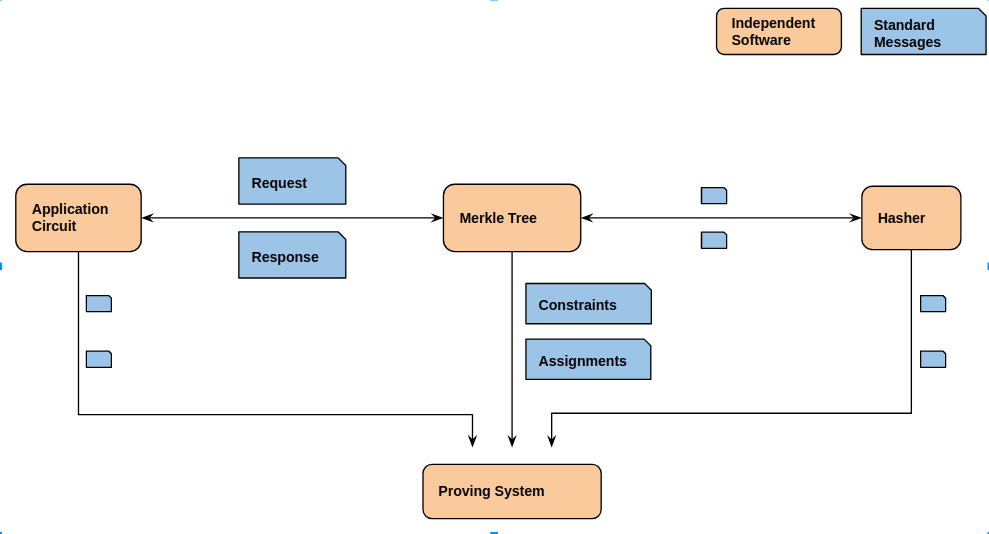
\includegraphics[width=\linewidth]{routine.png}
				\caption{The flow of interaction between existing libraries and the interface}
				\label{flow}
			\end{figure}

		\paragraph{Instance reduction.} 
		
        Points to include:
        - caller does not provide functionality to gadget and does not depend on specific implementation
        - gadget and caller both allocate variables
		
		\paragraph{Witness reduction.}
		
		r1cs in the format: a way to represent the constraints and a way to represent the assignment; and connection between components (gadgets), which actually are the public inputs. If we think of circuit as components, each component has a set of local inputs and "outgoing" inputs.
		
		So the interface solves two problems: 1/ interop between frameworks (front-ends) and proving systems (backends) 2/ composability of gadgets between different frameworks.
		
	
		
		\subsection{An MVP}
		
		
		
		\subsection{Specification}
        
        \paragraph{Interface Definition.}
        
        \paragraph{Request Call.}

        \paragraph{Callee Response.}

        \paragraph{Memory Allocation.}

        \paragraph{FlatBuffers.}

        \paragraph{Standard Format.}

		*use of flatboard
		
		- semantics; planned parametrization of the semantics.
		
		- format: can work with files (all messages instead of processing, can be written to file) for both instance / witness reduction, otherwise can work with memory 
		
		Each component has an interface; which can be invoked / instantiated / called with other components to make up the constraint system.
			- composibility of gadgets as there local variables / public ones (merkle tree has the leaf and root and invokes sha256)
		
		CRS is specific to proving system so the format does not handle the CRS portability
		
		we are thinking of implementing ZoKrates for the application layer and libsnark, bellman.  
		
		NOTE: some people think of functions, inputs and returned variables; others as circuits and gadgets.
		
		
		Issues: 1/ linear 

%=============================================================================
\section{Specification}

\enote{For now, maybe just remove this section, and leave only the narrative in the Architecture subsection, and the in-source comments?}
		
\paragraph{Interface Definition.}

	The interface is defined as a FlatBuffers schema that describes 
	the serialization of messages that the caller and callee can exchange.

	The FlatBuffers system includes a simple interface definition language,
	support for all common programming languages,
	a clear evolution path for future extensions of the standard,
	and the possibility of very efficient implementations.

	\anote{Add ref: https://google.github.io/flatbuffers/}

	The interface definition is provided in annex.

\paragraph{Request Call.}

\paragraph{Callee Response.}

	\paragraph{C API.}

\paragraph{Memory Allocation.}

\paragraph{File Format.}

\subsection{Interface Definition}



\subsection{Interface Definition}

	\lstinputlisting[
		caption=gadget.fbs - Interface definition,
		language=flatbuffers2,style=protobuf,
		label=gadget.fbs]{../gadget.fbs}

	\lstinputlisting[
		caption=gadget.h - C Interface,
		language=C++,style=protobuf,
		label=gadget.h]{../cpp/gadget.h}

\end{document}